\section{Наблюдатель пониженного порядка}

Исследуемая система описывается уравнениями:
\[
\begin{cases}
    \dot{x} = Ax + Bu, \\
    y = Cx + D,
\end{cases}
\]
где:
\begin{itemize}
    \item $x$ — вектор состояния системы,
    \item $u$ — входной сигнал (управление),
    \item $y$ — выходной сигнал.
\end{itemize}

Матрицы системы заданы следующим образом:

\[
A = \begin{bmatrix}
    5 & -7 & -5 & 1 \\
    -7 & 5 & -1 & 5 \\
    -5 & -1 & 5 & 7 \\
    1 & 5 & 7 & 5
\end{bmatrix}, \quad
B = \begin{bmatrix}
    5 \\
    7 \\
    1 \\
    9
\end{bmatrix}, \quad
C = \begin{bmatrix}
    0 & 1 & 0 & 0 \\
    1 & 0 & 0 & 0
\end{bmatrix}, \quad
D = \begin{bmatrix}
    4 \\
    2
\end{bmatrix}.
\]


\subsection{Исследование характеристик системы}

Найдём собственные числа матрицы $A$:
\[
    \sigma(A) = \{-8, 4, 8, 16\}.
\]

Проверим полные характеристики системы с помощью матриц наблюдаемости и управляемости:

\[
V = \begin{bmatrix}
    C \\
    CA \\
    CA^2 \\
    CA^3
\end{bmatrix}, \quad
    U = \begin{bmatrix}
    B & AB & A^2B & A^3B
\end{bmatrix}.
\]

Ранги матриц $V$ и $U$ равны 4:
\[
    \text{rank}(V) = 4, \quad \text{rank}(U) = 4.
\]

Матрицы являются полноранговыми, что означает, что система \textbf{полностью наблюдаема и управляема} по всем собственным числам. Из этого также следует, что система является \textbf{стабилизируемой и обнаруживаемой}.

\subsection{Синтез наблюдателя пониженного порядка}

Для наблюдателя пониженного порядка (который оценивает не все компоненты вектора состояния) выберем следующие матрицы $G$ и $Y$:

\[
G = \begin{bmatrix}
    -3 & 1 \\
    0 & -3
\end{bmatrix}, \quad
Y = \begin{bmatrix}
    1 & 0 \\
    0 & 1
\end{bmatrix}.
\]

Спектр матрицы $G$:
\[
    \sigma(G) = \{-3, -3\}.
\]

Условия для синтеза наблюдателя пониженного порядка аналогичны условиям для наблюдателя полного порядка, но используются матрицы меньшей размерности.

Решим уравнение Сильвестра для нахождения матрицы преобразования $Q$:
\[
GQ - QA = YC, \quad \rightarrow \quad Q = \begin{bmatrix}
    0.03 & -0.03 & 0.09 & -0.07 \\
    -0.02 & 0.05 & 0.07 & -0.09
\end{bmatrix}.
\]

Динамика наблюдателя описывается уравнениями:
\[
    \dot{z} = QAQ^{-1}z + QBu,
\]
\[
    \dot{\hat{z}} = G\hat{z} - Yy + (QB + YD)u.
\]

Для управления по обратной связи требуется оценка вектора состояния, которая формируется следующим образом:
\[
    u = K\hat{x}, \quad \hat{x} = \begin{bmatrix}
    C \\
    Q
\end{bmatrix}^{-1} \begin{bmatrix}
    y - Du \\
\hat{z}
\end{bmatrix}.
\]

\subsection{Синтез регулятора}

Для синтеза регулятора используем матрицы $Y$ и $G$ из предыдущего задания. Коэффициенты регулятора остаются неизменными:
\[
K = \begin{bmatrix}
    8.51 & -8.91 & -0.87 & -1.36
\end{bmatrix}.
\]


\subsection{Моделирование системы}

Проведём моделирование с начальными условиями:
\begin{itemize}
    \item Вектор состояния системы: $x(0) = \begin{bmatrix} 1 & 1 & 1 & 1 \end{bmatrix}^T$.
    \item Вектор состояния наблюдателя: $\hat{x}(0) = \begin{bmatrix} 0 & 0 & 0 & 0 \end{bmatrix}^T$.
\end{itemize}

\begin{figure}[H]
    \centering
    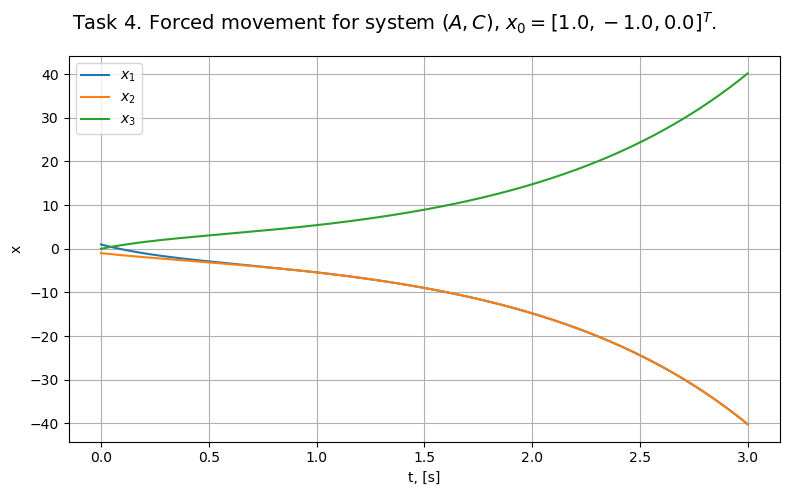
\includegraphics[width=0.7\textwidth]{../../plots/task_4_1.png}
    \caption{Состояние системы}
    \label{fig:task_4_state_system}
\end{figure}

\begin{figure}[H]
    \centering
    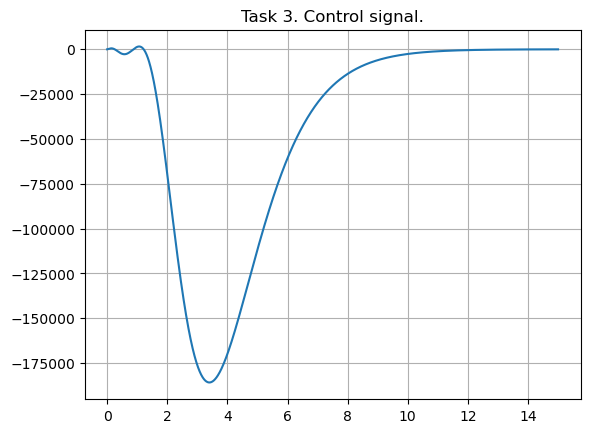
\includegraphics[width=0.7\textwidth]{../../plots/task_4_2.png}
    \caption{Управление регулятора}
    \label{fig:task_3_control_controller}
\end{figure}

\begin{figure}[H]
    \centering
    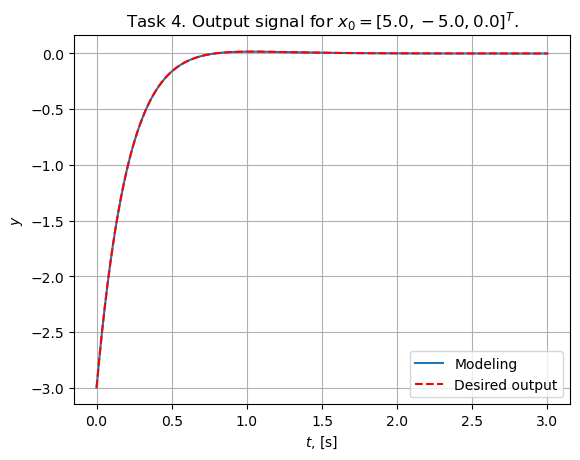
\includegraphics[width=0.7\textwidth]{../../plots/task_4_4.png}
    \caption{Ошибка наблюдателя}
    \label{fig:task_4_error_observer}
\end{figure}

Как видно из результатов моделирования, ошибка наблюдателя $e(t) = x(t) - \hat{x}(t)$ становится малой. Это означает, что наблюдатель почти сразу начинает точно оценивать состояние системы.


\subsection{Вывод}
В рамках данного задания мы синтезировали связку \textbf{модального наблюдателя пониженного порядка} и \textbf{регулятора}. Мы работали с системой, которая является \textbf{полностью наблюдаемой и управляемой}, что позволило нам свободно выбирать желаемые спектры как для наблюдателя, так и для регулятора. В отличие от полного наблюдателя, здесь мы отслеживали только \textbf{2 компоненты состояния системы} (из 4 возможных). Для этого был использован специальный подход к синтезу наблюдателя, основанный на решении \textbf{уравнения Сильвестра}, которое позволило найти матрицу преобразования $Q$.

Проведённое моделирование подтвердило успешную работу связки: наблюдатель корректно оценивал выбранные компоненты состояния системы, а регулятор обеспечивал стабилизацию системы в соответствии с заданными требованиями.

